%% ----------------------------------------------------------------
%% VideoPlayer.tex
%% ---------------------------------------------------------------- 

\chapter{Video Player}
\label{Chapter:Video Player}

\begin{preamble}
	Specific improvements to \gls{Videogular} were made in three areas: accessibility, compatibility and scrub bar extensions. Each area was conducted independently, and the contributions were readily accepted back into the \gls{Videogular} project or published as separate plugins. These were made to ensure that the \gls{Videogular} player met our accessibility needs and to add required features to the player.
\end{preamble}

\section{Introduction}

After reviewing the \gls{Videogular} project it was found that it was lacking in a number of aspects. Therefore to fulfil requirements such as \cref{Req:Keyboard accessibility} the following goals were identified for this part of the project:

\begin{itemize}
	\item investigate \gls{Videogular} to allow for its use within the new version of Synote
	\item improve the accessibility of \gls{Videogular} for users with reduced input options
	\item ensure that \gls{Videogular} was usable on as many devices as possible
	\item add the ability to mark locations on the \gls{scrub bar}
	\item produce a plugin to allow the display of statistical data along the \gls{scrub bar}
\end{itemize}

\section{Accessibility}
\label{Section:Accessibility}
\gls{Videogular} has the option to display HTML controls for the video player, replacing the browser's built-in controls. However, when the project began there was no way for the user to access these controls without a mouse. The main problem was that the controls did not identify themselves as interactive elements, and so could not be `focused' (selected with the tab key). This also prevented them from being picked up by a screen reader.

\subsection{Design and Implementation}
Some online video players allow the player as a whole to be focused, and then controlled with various keyboard shortcuts. The problem with this method is that accessibility aids, such as screen readers, will not have information on these controls, and so users of those technologies will require further instruction. It is also not accessible to users of a clicker, who can only press one key and so require individually focusable controls.

Instead, the controls were made individually focusable by using semantic markup where possible, and \gls{ARIA} attributes otherwise. When a control is in focus, a visual indicator is displayed to highlight it. Buttons can then be pressed using the space bar (\fref{Figure:Accessibility/Screenshots/Button}); the scrub bar can be moved using the left and right arrow keys (\fref{Figure:Accessibility/Screenshots/ScrubBar}); and the volume can be adjusted using the up and down arrow keys when the mute button is focused (\fref{Figure:Accessibility/Screenshots/Volume}).

\begin{figure}
	\begin{subfigure}[]{\textwidth}
		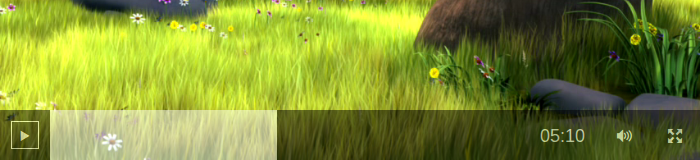
\includegraphics[width=\textwidth]{accessibility/button}
		\caption{The controls with the play button focused. In this state, pressing the space bar plays or pauses the video.}
		\label{Figure:Accessibility/Screenshots/Button}
	\end{subfigure}
	\begin{subfigure}[]{\textwidth}
		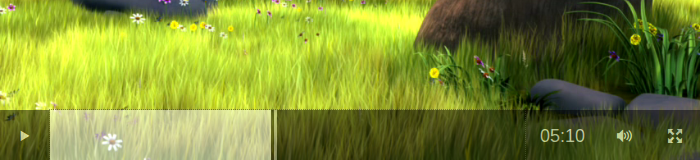
\includegraphics[width=\textwidth]{accessibility/scrub-bar}
		\caption{The controls with the scrub bar focused. In this state, pressing the left or right arrow keys skips backwards or forwards in the video.}
		\label{Figure:Accessibility/Screenshots/ScrubBar}
	\end{subfigure}
	\begin{subfigure}[]{\textwidth}
		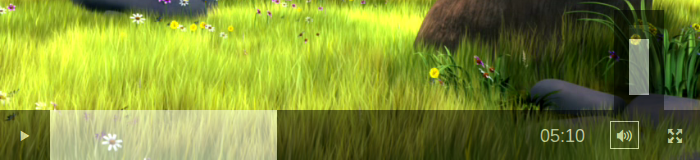
\includegraphics[width=\textwidth]{accessibility/volume}
		\caption{The controls with the mute button focused. In this state, the volume control appears, pressing the space bar toggles mute, and the up and down arrow keys change the volume.}
		\label{Figure:Accessibility/Screenshots/Volume}
	\end{subfigure}
	\caption{Screenshots of the accessibility improvements made to \gls{Videogular}'s HTML controls.}
	\label{Figure:Accessibility/Screenshots}
\end{figure}

\subsection{Conclusions}

This solution is not completely clicker-accessible, but could be made so by introducing buttons to skip forwards or backwards, and to raise or lower the volume. It is a significant improvement on the original state, as keyboard users can now use the player. The improvements were submitted to the \gls{Videogular} project\footnote{\url{https://github.com/2fdevs/videogular/pull/108}}, and are now part of \gls{Videogular} 0.6.1.

\section{Compatibility}
\label{Section:Compatibility}

One of the main focuses during this part of the project was to make sure the application was compatible with a range of platforms, operating systems and devices (\cref{Req:Browser compatibility}, \cref{Req:OS compatibility}). The first challenge was to ensure that the player and overlay displayed correctly at a variety of resolutions and screen/window sizes.

Apple iPhones caused a problem, as Safari forces the video to be played in full-screen mode. This is a design choice and there is no way to play the video inline, as directives to do this are ignored by the browser.

This meant that the video paused at the correct time but as the video is in the native player the overlay was not visible unless the player was closed. There is no way of notifying the user that this needs to be done. A possible solution involves telling the user to quit out of the video when it is paused so they may answer the question, but this is not very convenient. However, this is not an issue on iPads.

Android phones correctly interpret the inline directive and will play the video properly, so the questions overlay is correctly applied and usable. This has been the primary focus of testing on mobile devices as it represents a very large portion of the market.

The overlay which displays questions appears above the video and obstructs it. Placing the overlay in the middle of the screen requires complex \gls{CSS} to correctly locate it on small screens. There are still some issues with the pop-up location on some mobile devices where the browser reports an incorrect screen size. Until these devices are compliant with the specification, it is too time consuming to fix each individual case.

All tablets tested, running iOS or Android, display the pop-up correctly. This is because they allow a video to be played inline and have content appear above the video. They also do not need additional \gls{CSS} to position the pop-up as they normally have laptop-size screens (\textgreater 1024 pixels wide) which do not require any video scaling. (The video was 700 pixels wide at its maximum size.)

The best user experience with this application is using it on a desktop with an up-to-date browser. This will definitely work and display as intended. As the screen size of the device gets smaller the user experience is significantly reduced as the video and poll overlay will be much smaller than recommended. To support a number of browsers and operating systems a range of video formats are supplied to the \gls{Videogular} plugin so that the browser can pick one that is supported.

\section{Scrub Bar Extensions}
\label{Section:Scrub Bar Extensions}

\gls{Videogular} has been designed and implemented in such a way as to allow for directive-based plugins to be developed to extend its functionality. When using the \gls{Videogular} Controls, the native browser controls are replaced with an HTML based interface. All our interface changes are for \gls{Videogular} Controls, not the native browser controls.

The team behind \gls{Videogular}, 2fdevs, are actively seeking members of the community to develop new plugins for their system, and so were willing to discuss the plugins and their architectural design.

\subsection{Videogular Cuepoints}
\label{Subsection:vgCuepoints}
\gls{Videogular} Cuepoints is a \gls{Videogular} plugin for displaying `cuepoints', marks on the scrub bar which can be positioned at different times. For example, cuepoints could indicate the start of a section in the video, or (in this case) a time when a pop up will appear.

\subsubsection{Design and Implementation}
Like the rest of Videogular Controls, each cuepoint is represented by an HTML element which is positioned using \gls{CSS}. This allows users of the plugin to style them with their own stylesheets.

Cuepoint positions are specified in the \texttt{config} object which is given as a parameter to cuepoints, and a stylesheet for a custom theme can be specified in the same way.

One problem found during implementation was that the cuepoints cannot be displayed before the video has begun playing. This is due to \gls{Videogular} not setting the video length variable until the video plays, and so this variable cannot be used to calculate the positions of the cuepoints until then.

\subsubsection{Further Work}
In future, the ability to specify a different \gls{CSS} class for each cuepoint could very easily be added, allowing visual differentiation of the markers. It would also be useful to make the cuepoints more accessible, for example by providing alternative text for screen readers.

There may also be scope for investigating why the \gls{Videogular} player does not set the length variable before it starts playing and if there are any fixes for this. Initial investigation concluded that until the video starts playing it is impossible to determine the length of the video. However, loading the video via a second hidden \gls{HTML5} element and playing it may give access to the video length.

\subsection{Videogular Heatmap}
\gls{Videogular} Heatmap is a \gls{Videogular} plugin for giving areas of the scrub bar different colours. In our examples this is used to give a visual representation of the number of times each section of the video has been watched.

\subsubsection{Design and Implementation}
An early design decision was to use \gls{CSS} to colour the sections as this would allow different colours to be specified (see \cref{Req:Use of colour}). This also would allow developers to develop their own colour schemes with meanings if they desired.

Sections and colours can be specified in a \texttt{config} object which is given as a parameter when the heat map is used.

The format for defining the configuration parameters was made consistent with Videogular Cuepoints (see \autoref{Subsection:vgCuepoints}) to improve usability.

The same issue that was encountered with the Cuepoints plugin, which prevents display until the video plays, was a problem for the heat map plugin. This is less of an issue for this plugin as the colouring does not have any context for a user until they have watched the video.

An extra option that was added for improved accessibility was the ability to label each heat map section with the frequency. Extra hidden text was added so that a screen reader user could still access all the data shown in the heat map.

\section{Conclusions}

Several improvements to \gls{Videogular} were made during the course of the project, primarily focussing on accessibility. With these changes the \gls{Videogular} player is now accessible to users who only navigate websites using the keyboard. All changes made have been adopted by the \gls{Videogular} project. Compatibility with a number platforms and devices was reviewed and the only major problem found was that Safari forces video to be full-screen on iPhones.

We created two \gls{Videogular} plugins to allow us to display markers and statistical data on the \gls{scrub bar}. Both of these have been designed for use in our example websites, cuepoints for points where questions appear and the heat map to demonstrate how often sections of a video have been watched.


